\appendixitem{DEFINITIONS}

DEFINITION 1. A combinatorial graph (or simply a graph, if there is no risk of confusion) is a pair \((\mathrm{A},\mathrm{S})\) , where \(\mathrm{S}\) is a set and \(\mathrm{A}\) is a subset of \(\mathfrak{P}(\mathrm{S})\) consisting of sets with two elements.

Let \(\Gamma = (A, S)\) be a graph. The elements of A are called the edges and those of S the vertices of \(\Gamma\) ; two vertices are said to be joined if \(\{x, y\}\) is an edge. A vertex is called terminal if it is joined to at most one vertex, and a ramification point if it is joined to at least three vertices.

In accordance with the general definitions (Sets R. §8), an isomorphism from the graph \(\Gamma\) to a graph \(\Gamma' = (A', S')\) is a bijection from \(S\) to \(S'\) that takes \(A\) to \(A'\) . A graph \(\Gamma' = (A', S')\) is called a subgraph of \(\Gamma\) if \(S' \subset S\) and \(A' \subset A\) ; \(\Gamma\) is called a full subgraph of \(\Gamma\) if \(S' \subset S\) and \(A' = A \cap \mathfrak{P}(S)\) . It is clear that every subset of \(S\) is the set of vertices of exactly one full subgraph of \(\Gamma\) .

To make the arguments easier to follow, we represent a graph by a diagram having points corresponding to the vertices, two points being joined by a line if and only if the vertices they represent are joined in the graph. For example, the diagram

\pandocbounded{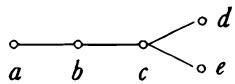
\includegraphics[keepaspectratio]{images/part001_959a1795.jpg}}

represents a graph whose vertices are \(a, b, c, d, e\) and whose edges are \(\{a, b\}\) , \(\{b, c\}\) , \(\{c, d\}\) and \(\{c, e\}\) .

